\section{Motivation}
\label{sec:intro:motivation}

In this section, we first study the need of inductive biases in
machine learning. Then we analyze where the current deep learning
models can get inductive biases from, and finally we highlight some
open problems that this thesis addresses about inductive biases on
deep linguistic structured prediction.

\subsection{Generalization: The Need for Inductive Bias}
\label{ssec:intro:need-of-bias}

Any system~(natural or artificial) that makes general inferences on
the basis of particular and limited data must constrain its hypotheses
in some way before observing data. With limited observations and
resources~(time, memory, energy), our human intelligence of
generalizing to new environments makes us efficiently learn when
interacting with the world and other human beings. This efficiency
largely depends on many {\bf inductive biases} from human
intelligence~\citep{Gershman2021WhatMU}, which are potentially helpful
for machine intelligence. According to extensive cognitive
studies~\citep{Spelke1990PrinciplesOO,Bienenstock1996CompositionalityMP,Rehder2003ACT,harlow1949formation,
  Lake2016BuildingMT,Gershman2021WhatMU}, there are many key inductive
biases for human intelligence, such as compositionality, causality,
learning to learn, and so on. We are not meaning machine intelligence
should mimic the human intellgence. Instead, we arguably that mean
those key human indutive biases under limited observation and
resources may inspire us to design the machine intelligence.

On the machine intelligence side, as the no-free-lunch theorem for
machine learning said~\citep{baxter2000model,wolpert1995no}, inductive
biases that influence hypothesis selection is necessary to obtain
generalization. Tom M Mitchell argues that
inductive biases constitue the heart of generalization and indeed a
key basis for learning itself~\citep{mitchell1980need}.

As the supervised learning setting shown in
\autoref{fig:intro-hypothesis}, $\mathcal{H}$ refers to machine
learning model families, including those deep learning models.
According to the universal approximation theorem, properly
parameterized neural network can represent any functions. The task of
finding a hypothesis $h$ is reduced to estimating the nerual network
parameters by fitting the training data. However, the labaled data is
usually noisy and cannot represent the whole distribution of the real
data distribution, let alone new input data with distribution shift.
Hence, preferences on how to choose the hypothesis class
$\mathcal{H}$ and how to select the $h$ is necessary to generalize to
new data.

\begin{figure}[!th]
\centering
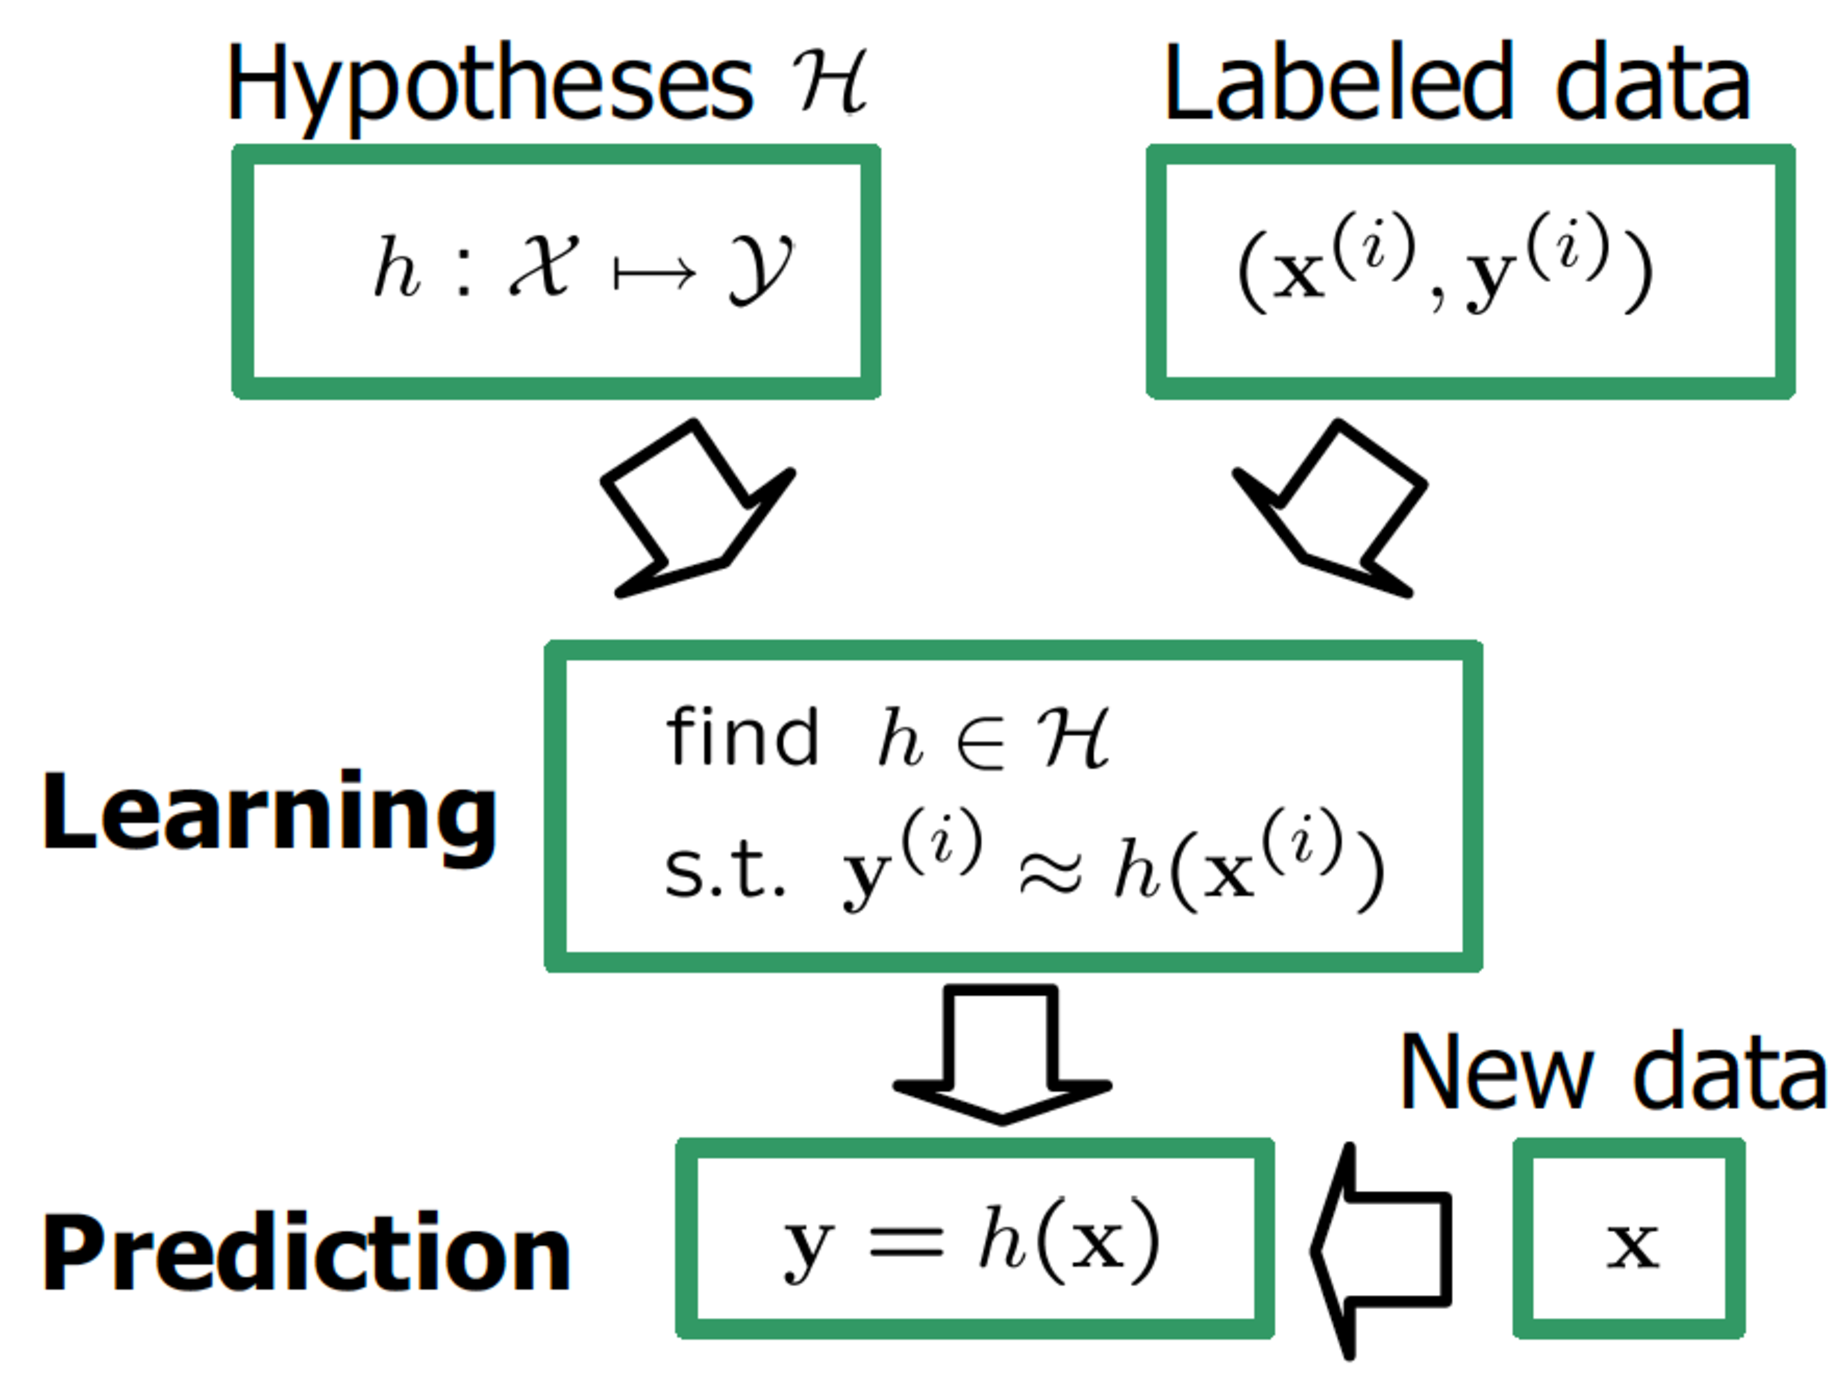
\includegraphics[width=0.80\textwidth]{supervised-learning-hypothesis.pdf}
\caption{\label{fig:intro-hypothesis}Hypothesis, Generatioalization in
  Supervised Learning Setting\todo{Current fig is directly copied from
    Ben Taskar's thesis, redraw it}}
\end{figure}

In this thesis, following the definition of \kw{bias}
in~\cite{mitchell1980need}, we refer \kw{indutive bias} as follows:

\begin{proof}[\kw{Definition of Inductive Bias}]
  \label{def:bias}
  `Any biases for choosing one generalization over another, other than
  strict consistency with the observed training instances'.
\end{proof}

\subsection{Hypothesis Class and Hypothesis: The Origins of Inductive Biases}
\label{ssec:intro:bias-source}
Inductive biases are widely used in the whole history of machine
learning. As the supervised learning setting in
\autoref{fig:intro-hypothesis} and the definition inductive biases in
~\autoref{def:bias}, inductive biases are mainly from hypothesis class
selection and how to find the specific hypothesis $h$.

According to the two goals, we organize the origins of inductive
biases in two parts:

\Paragraph{Goal 1: Deciding hypothesis class $\mathcal{H}$}

\begin{itemize}
\item \kw{Model Family} Different model family can represent different
  hypothesis classes. For example, generalized linear models such as
  logistic regression and support vector machines, can only support
  arbitary linear decision boundaries. \todo{add more models}.


\item \kw{Feature Engineering and Kernel Methods} \todo{Inductve
    biases also can be found in feature engineering, } However, not
  every training data are linear seperable. One solution to this
  kernal-based SVM. The design of kernel is inductive bias.

\item \kw{Neural Architecture and Representation Learning} What's
  more, inductive bias are widely used in modern deep learning
  architeuctures, which also decides the hypothesis space.  For
  example, translation invariance for convolutional neural
  networks~(CNN) and pooling, and recurrent assumption of recurrent
  neural networks~(RNN), equivariance over permutation for neural
  graph networks~(GNN), positional encoding for word orders in
  Transformer.  \todo{geometry deep learning}
\end{itemize}

\Paragraph{Goal 2: Finding the specific hypothesis $h$}
\begin{itemize}
\item \kw{Optimization} Even in existed computing-heavy and data-heavy
  scenarios, inductive biases are widely used in well-known deep
  learning techniques. For example, smoothness assumption in
  optimization method, such as Stochostic gradient decent, which was
  proofed as another inductive bias to have better generalization.
  \todo{SGD generalization,smoothness} \todo{Optimization will control
    the bias shift during learning}

\item \kw{Training Data} It is often the case that available datasets
  do not exactly represent the data distribution of interest.  One
  particularly problematic case is when the dataset is biased in some
  way against a particular demographic group, which often leads to
  model predictions that unfairly disadvantage members of that
  group.


%For example, naturally occurring data will often
%  underrepresent minority groups, so systems can do well on average
%  while having high error rates on these groups (Blodgett et al.,
%  2016; Tatman, 2017; Buolamwini and Gebru, 2018; Sap et al.,
%  2019). Datasets may also recapitulate stereotypes tied to historical
%  injustices, which incentivizes models to learn these very
%  stereotypes to achieve the best test accuracy (Zhao et al., 2017,
%  2018; Rudinger et al., 2018). Training data collected from current
%  users of a system will likely be skewed towards users for which the
%  system works well, leading to a feedback loop in which underserved
%  users become increasingly underrepresented in the training data
%  (Hashimoto et al., 2018). In many cases, avoiding these types of
%  biases can be thought of as optimizing a worst-case objective in
%  which an  adversary  may change the data distribution to include
%  more minority group members, or include more examples that invert
%  stereotypes. While this thesis does not focus on preventing bias
%  against underrepresented minorities, we believe it is an important
%  motivating case for work on robustness.

\todo{Data augmentation for different pertubation}

\todo{Realistic distribution shift}

\item \kw{Inference Algorithm} Combinatorial Optimization approaches,
  such as graph cuts, partitions, bipartie mactching, dynamic
  programming can also be involved during the hypothesis learning,
  which will also constrain the learning.  In this thesis, we mainly
  focus on representation learning, for inference, we use the existing
  methods, such as greedy, maximum spanning connected graph, dynamic
  programming for CKY parsing.

\end{itemize}

In this thesis, we mainly study inductive biases from nerual
architecture and the corresponing represetion learning.

\subsection{Inductive Biases for Deep Lingusitic Structured
  Prediction}
\label{ssec:intro:bias-dsp}

Towards flexible out-of-distribution and systematic generalization,
the search for appropriate inductive biases is also necessary for
deep linguistic structured prediction.

Given an observation $x \in \mathcal{X}$~(natural language text), define
a structured prediction $y \in \mathcal{Y}(x)$ as $y=f(x)$. Here $y$ is
a structured symbolic representation for $x$, e.g., $y$ cound be a
sequence of part-of-speech tagging, constituent tree or dependency
tree, or $y$ can a broad-coverage meaning representation, like AMR,
UCCA, or an application-specific representation like frame-based
dialog state~\cite{bobrow1977gus}. To represent the target function
$f(x)$, we adopt the popular energy-minimization strategy by defining
$f(x)$ as the minimizer of an auxiliary energy optimization problem.
\begin{equation}
\label{eq:argmin}
f(x) = \argmin_{y \in \mathcal{Y}(x)} E(x, y),
\end{equation}
where $E(x,y)$ is a scoring function to represent the energy between
$x$ and different candidate output structures $y$.

In many NLP applications, the candidate output set $\mathcal{Y}(x)$ is
typically finite but exponentially large, and its size may depend on
the input $x$. To render either exact or approximate optimization of
energy-minimization in Equation~\ref{eq:argmin}, how to model the
representation of \IN~and~\OUT, and the interactions between them are
challenging problems. Practitioners typically employ energy functions
with specific factorization structures to design efficient algorithms,
by assuming the whole energy $E(x, y)$ can be decomposed as a sum of
\textbf{factors} $c \in C$. A popular choice to represent the
facortization is to index both $x$ and $y$ as a set of sub components
$x=(x_{1},..., x_{i},.... x_{N})$ and $y=(y_{1},...y_{j},...y_{M})$.

In AMR parsing as shown in Figure~\ref{fig:intro-dog-amr},
$x_{i}$ can be each word or multi-word expression in a sentence, while
$y_{j}$ can be single AMR node and relation.  For dialog state
tracking in Figure~\ref{fig:label-example}, $x_{i}$ is an utterance in
the dialog, while $y_{i}$ is the value for each intent and slot in the
predicted frames.

The interdependence assumptions between those subcomponents in $x$ and
$y$ are key in structured prediction model. In the
\autoref{chap:background}, we show various representation formalism
~(such as graphic models), structured learning~(max-margin framework)
and inference approaches~(dynamic programming, integer linear
programming) to modeling the interdependence. Inductive biases can be
designed in all the three key aspects.

In this theis, for representation formalism for factorization
assumption, we always assume the independent factorization paradigm,
where each factor $c$ only depends on a subset of $y$ components
$y_{c}$ and the aligned $x$ components~(anchors)~$x_{c}=a(y_{c})$. In
another word, the output part $y_{c}$ in factor $c$ is independent
with output part $y_{c^{\prime}}$ in another factor $c^{\prime}$. Here,
$a(y_{c})$ is the alignment model to find how independent output parts
$y_{c}$ are anchored to the constituents of the observation $x$, thus
the prediction of each $y_{c}$ are independent with each other, and
can be locally decided by its aligned anchors.

\begin{equation}
    \label{eq:independent-factor}
    \begin{split}
    E(x, y) & =\sum_{c \in C} E(x, y_{c}) = \sum_{c \in C}E(a(y_{c}), y_{c})  \\
    f(x) & = \argmin_{y \in \mathcal{Y}(x)} E(x, y), \\
         & = \argmin_{y \in \mathcal{Y}(x), a \in A} E(a, x, y),
    \end{split}
\end{equation}

Hece, this simple independent factorization decompose the structured
learning into decomposed local learning. More importantly, it also
makes the inference intractable, thus can be easily involved in the
end-to-end neural network training.

Using the AMR Paring in \autoref{fig:intro-dog-semantics} as an
continue example, by allowing the input constituent $x_{c}$ mapped
into an empty output $y_{c}=\phi$, the design of independent
factorization will first segment the output $y$ into small parts
$y_{c} \in seg_{out}(y)$, then find the anchors $x_{c}$ for each
$y_{c}$ from the candidate decomposition set $seg_{in}(x)$. For
example, one of the segmented $y_{c}$ in
Figure~\ref{fig:intro-example} is a pre-categorized sub-graph
`(possible-01 :polarity -)', and $a(y_{c})$ of that is the anchor word
`cannot'. However, the words `the', 'from' are mapped to empty nodes.
During inference, we can directly produce $y_{c}$ for all candidates
segments in a new sentence as shown in
Figure~\ref{fig:independent-example}. We first prepate a list of
candidate anchors $seg_{in}(x)=\{${`The', `dog', `found', `the',
  `bone', `it', `hide'$\}$, then the model will produce the
  independent prediction $y_{c}$ of each anchor as
  $\{\phi,\text{`dog'}, \text{`find-01'}, \phi, \text{`bone'},\text{`it'},
  `hide'\}$, then we assemble the non-empty $y_{c}$ by predicing the
  relations between each other and finally forms \OUT via
  postprocessing\footnote{The post-processing include mergeing
    coreference nodes~(as the `dog' and `it'), adding other
    attributes}.

  Hence, in the independence factorization setting, the problem is
  reduced into three challenges:
\begin{itemize}
\item How to decompose the output $y$ into a set of independent parts
  $y_{c}$.

\item How to derive the aligned input $a_{y_{c}}$.

\item How to model the representation of $a_{y_{c}}$ and $y_{c}$, thus
  computing the energy score $E(x_{a(y_{c})}, y_{c})$.
\end{itemize}

In this thesis, the first question on independently decomposing $y$ is
either straightforward or has been resolved by previously existing
methods in our studied tasks. We mainly focus on the remaining
challenges on modeling alignment and representation learning.

%%% Local Variables:
%%% mode: latex
%%% TeX-master: "../../thesis-main.ltx"
%%% End:
